\documentclass[draft]{penrose}

\usepackage{mathsphystools}
\usepackage{thmstyles}
\usepackage{graphicx}
\graphicspath{{images/}}

\usepackage{tikz}

\setlist[enumerate,1]{label=(\roman*)}
\setlist[enumerate,2]{label=\alph*.}

\newcommand{\oB}{B}
\newcommand{\cB}{\overline{B}}

\title{Norms, Metrics and Topologies}
\subtitle{Lecture Notes}
\author{Rashid M. Talha}
\affiliation{School of Natural Sciences, NUST}
\date{\today}
\begin{document}

\maketitle
\begin{center}
  \textbf{Notes.}\par
  First delivered at NUST during the fall semester, 2022--23. Currently incomplete.
\end{center}

\section{Review, terminology, and notation}
BASICS OF SETS. SOME NOTATION.

BASICS OF FUNCTIONS. THE INVERSE-IMAGE (PRE-IMAGE). THE EXISTENCE AND UNIQUENESS OF THE INVERSE. SOME NOTATION.

BASICS OF INEQUALITIES.

RECAP OF THE DEFINITION OF SEQUENCES AND THEIR LIMITS. DEFINITION OF A CAUCHY SEQUENCE.

\section{Normed vector spaces}
\begin{ndfn}[Norm]
  Let $V$ be a vector space over $\R$. A norm on $V$ is a function $\norm{\cdot}:V\to\R$ with the following properties
  \begin{enumerate}
  \item $\norm{v} = 0 \iff v =0$, for $v \in V$, \hfill (definiteness)
  \item $\norm{\lambda v} = \abs{\lambda}\norm{v}$, $\forall \lambda \in \R$ and $\forall v \in V$, \hfill (absolute homogeneity)
  \item $\norm{u+v} \leq \norm{u} + \norm{v}$, $\forall u,v \in V$. \hfill (triangle inequality)
  \end{enumerate}
\end{ndfn}

\begin{ndfn}[Normed space]
  Let $V$ be a vector space, and let $\norm{\cdot}$ be a norm on $V$. The pair $(V, \norm{\cdot})$ is called a normed (vector) space.
\end{ndfn}

Some authors give a slightly different, but equivalent definition of the norm.

It should be clear from the definition that the vector space structure on $V$ is a necessity, since the axioms of being a norm rely on the existence of $0 \in V$ (the additive identity), scalar multiplication, and addition. We shall focus on the case where the underlying field is the real numbers, $\R$, however, an analogous theory can be developed in the case of other fields, for example, the complex numbers $\C$.

The idea behind defining a norm $\norm{\cdot}$ is that $\norm{x}$ should give us a measure of the \emph{magnitude} of the vector $x$. And magnitudes (or lengths) should be non-negative. So, the norms should be non-negative valued. The next result confirms this property. Some authors directly require $\norm{\cdot}:V\to[0,\infty)$, which simply gives the following proposition the status of an axiom.

\begin{nprop}[Non-negative valued]
  Let $\norm{\cdot}:V\to\R$ be a norm on $V$. Then, $\forall x \in V, \norm{x} \geq 0$.
\end{nprop}
\begin{proof}
  Observe the following
  \begin{equation*}
    0
    \overset{\text{(i)}}{=} \norm{0}
    = \norm{x+(-x)}
    \overset{\text{(iii)}}{\leq} \norm{x} + \norm{-x}
    \overset{\text{(ii)}}{=} \norm{x} + \abs{-1}\norm{x}
    = \norm{x} + \norm{x}
    = 2\norm{x}.
  \end{equation*}
  So, $2\norm{x} \geq 0$ for all $x \in V$, from which we conclude that $\norm{x} \geq 0, \forall x \in V$.
\end{proof}

Note that this proof works even when $V$ is a vector space over a general field $K$.

\begin{nprop}[Normed subspace]
  Let $(X, \norm{\cdot})$ be a normed space, and let $Y$ be a vector subspace of $X$. Then, $(Y, \norm{\cdot})$ is also a normed space, using the same norm as $X$. $(Y, \norm{\cdot})$ is called the normed subspace of $(X, \norm{\cdot})$. More precisely, this proposition claims that the function $N:Y \to \R$ with $N(y) \coloneq \norm{y}$, for all $y \in Y$, is a norm.
\end{nprop}
\begin{proof}
  Exercise.
\end{proof}

\begin{nex}
  Let $\norm{\cdot}_a$ and $\norm{\cdot}_b$ be any two norms on $V$. Do the following satisfy the definition of a norm
  \begin{enumerate}
  \item $\norm{\cdot}_a$ + $\norm{\cdot}_b$
  \item $\lambda\norm{\cdot}_a + \mu\norm{\cdot}_b$, for $\lambda, \mu \in \R$.
  \item $\norm{\cdot}_a \times \norm{\cdot}_b$
  \item $\sqrt{\norm{\cdot}_{a}}$
  \item $\norm{\left(\norm{\cdot}_b\right)}_{a}$, with the appropriate changes in domain.
  \end{enumerate}
\end{nex}

Let $V$ be a finite dimensional vector space over $\R$. Then, a result from introductory linear algebra shows that $V \cong \R^n$. Define the family of functions $\norm{\cdot}_{p}:\R^n \to \R$,
\begin{equation*}
  \norm{x}_{p} \coloneq \left(\sum_{j=1}^{n} \abs{x_j}^{p}\right)^{1/p}
  \quad\text{and}\quad
  \norm{x}_{\infty} \coloneq \max \set{x_1, \dots, x_n},
\end{equation*}
for $p \in [1,\infty)$ and $x = (x_1, \dots, x_n) \in \R^n$. Despite the suggestive notation, we have not yet claimed that these functions are valid norms.

\begin{nex}
  Show that the functions $\norm{\cdot}_{1}$ and $\norm{\cdot}_{\infty}$, are norms on $\R^n$.
\end{nex}

\begin{nex}
  Show that the function $\norm{\cdot}_{p}$, for $p \in (1,\infty)$, satisfies property (i) and (ii) of being a norm.
\end{nex}

\begin{remark}
  Indeed it will be shown later that $\norm{\cdot}_{p}$ is a norm on $\R^n$, but it will be extremely difficult to show directly that it also satisfy the triangle inequality. In order to establish the triangle inequality we will have to develop an alternative method.
\end{remark}

\begin{ndfn}
  Let $(V, \norm{\cdot})$ be a normed space. We define
  \begin{enumerate}
  \item the open unit ball: $\oB_{V} \coloneq \set{v \in V : \norm{v} < 1}$
  \item the closed unit ball: $\cB_{V} \coloneq \set{v \in V : \norm{v} \leq 1}$
  \end{enumerate}
\end{ndfn}
These sets depend on the norm that is being used on $V$.

The closed unit balls produced by the $\ell_{1}$, $\ell_{2}$, and $\ell_{\infty}$ norms on $\R^2$ are shown below.
\begin{center}
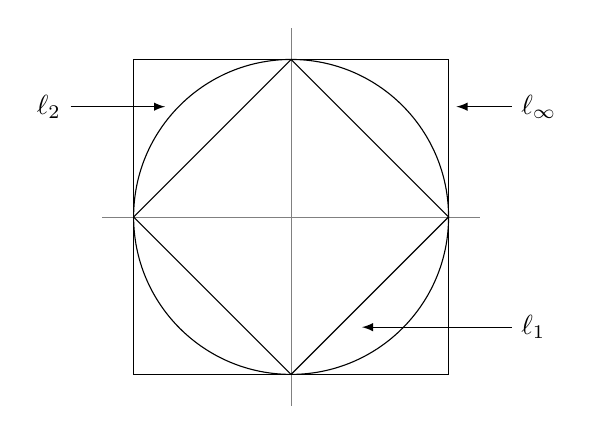
\begin{tikzpicture}[scale=2]
  \draw[help lines] (-1.2,0) -- (1.2,0);
  \draw[help lines] (0,-1.2) -- (0,1.2);
  \draw circle (1cm);
  \draw (1,0) -- (0,1) -- (-1,0) -- (0,-1) -- cycle;
  \draw (1,1) -- (-1,1) -- (-1,-1) -- (1,-1) -- cycle;

  \draw[-latex] (1.4, 0.7) node[anchor=west] {$\ell_{\infty}$} -- +(-0.35, 0);
  \draw[-latex] (-1.4, 0.7) node[anchor=east] {$\ell_{2}$} -- +(0.6, 0);
  \draw[-latex] (1.4, -0.7) node[anchor=west] {$\ell_{1}$} -- +(-0.95, 0);
\end{tikzpicture}
\end{center}

\begin{ndfn}[Convex sets]
  Let $V$ be a vector space. A set $X \subseteq V$ is called convex if $\forall x,y \in X$, and $\forall \lambda \in (0,1)$
  \begin{equation*}
    (1-\lambda) x + \lambda y \in X.
  \end{equation*}
\end{ndfn}
Geometrically, this is saying that $X$ is convex if the line segment joining any every pair of points in $X$, lies entirely within $X$.

\begin{ndfn}[Convex functions]
  A function $f : A \subseteq \R \to \R$ is called convex if $\forall x,y \in A$, and $\forall \lambda \in (0,1)$
  \begin{equation*}
    f\left((1-\lambda) x + \lambda y\right) \leq (1-\lambda) f(x) + \lambda f(y).
  \end{equation*}
\end{ndfn}
Therefore, a function is convex exactly when its graph lies beneath (or along) the line segment joining any two points on the graph. Common examples of convex functions are $x^2$ and $e^x$ on $\R$.

\begin{nprop}
  Let $(V, \norm{\cdot})$ be a normed space. The sets $\oB_{V}$ and $\cB_{V}$ are convex.
\end{nprop}
\begin{proof}
  We shall prove this for $\cB_{V}$. Take $a, b \in \cB_{V}$, and $\lambda \in (0,1)$. Then,
  \begin{equation*}
    \norm{(1-\lambda) a + \lambda b}
    \leq (1-\lambda) \norm{a} + \lambda \norm{b}
    \leq (1-\lambda) + \lambda
     = 1.
  \end{equation*}
  Therefore, $(1-\lambda) a + \lambda b \in \cB_{V}$. So, $\cB_{V}$ is convex.

  The proof for the convexity of $\oB_{V}$ is analogous.
\end{proof}

\begin{nprop}
\label{thm:convexity}
  Suppose $f \in C^2 ((a,b))$ and $f \in C^1 ([a,b])$. If $f''(x) \geq 0$, for all $x \in [a,b]$, then $f$ is convex on $[a,b]$.
\end{nprop}
\begin{proof}
  The proof is left as an exercise to the reader.
\end{proof}

\begin{nlemma}
  The function $f : \R \to [0,\infty)$ with $x \mapsto \abs{x}$ is convex.
\end{nlemma}
\begin{proof}
  To be completed. Uses the MVT.
\end{proof}

\begin{nlemma}
  The function $f : [0,\infty) \to \R$ with $x \mapsto x^p$ is convex, $\forall p \in [1,\infty)$.
\end{nlemma}
\begin{proof}
  The given function is a polynomial, so it is infinitely differentiable, with
  \begin{equation*}
    f''(x) = p(p-1)x^{p-2}.
  \end{equation*}
  Now,
  \begin{equation*}
    p \in [1,\infty), x \in [0,\infty) \implies p, (p-1), x, x^{p-2} \geq 0.
  \end{equation*}
  Therefore, $f''(x) \geq 0$, for all $x$ in the given domain.

  Proposition (\ref{thm:convexity}) then states that $f(x) = x^p$ is convex.
\end{proof}

\begin{nlemma}
  If $f: A \to B$ and $g: B \to C$ are convex functions, then $g \circ f : A \to C$ is also convex.
\end{nlemma}
\begin{proof}
  Take $x,y \in A$ and $\lambda \in (0,1)$. Then,
  \begin{align*}
  (1-\lambda) (g \circ f)(a) + \lambda (g \circ f)(b)
  &= (1-\lambda) g(f(a)) + \lambda g(f(b))\\
  &\geq g\left((1-\lambda) f(a) + \lambda f(b)\right)\\
  &\geq g\left(f\left((1-\lambda) a + \lambda b\right)\right)\\
  &= (g \circ f)\left((1-\lambda) a + \lambda b\right).
  \end{align*}
  Therefore, $(g \circ f)$ is convex.
\end{proof}

Combining these lemmas, we obtain that $\forall p \in [1,\infty)$, $x \mapsto \abs{x}^{p}$ is a convex function. In other words, $\forall x,y \in \R$, and $\forall \lambda \in (0,1)$,
\begin{equation*}
  \abs{(1-\lambda) x + \lambda y}^{p} \leq (1-\lambda) \abs{x}^{p} + \lambda \abs{y}^{p}.
\end{equation*}

Now, we consider a norm-like function that is required to satisfy all the properties except the triangle inequality. If we require the \emph{closed balls} produced by this function to be convex, then we find that it also ends up satisfying the triangle inequality. So, the next result allows us to establish the triangle inequality by checking the convexity of the induced closed balls.

\begin{nthm}
\label{thm:norm-convex-triangle}
  Let $V$ be a vector space, and consider a function $N : V \to [0,\infty)$ with
  \begin{enumerate}
  \item $N(v) = 0 \iff v =0$, for $v \in V$,
  \item $N(\lambda v) = \abs{\lambda}N(v)$, $\forall \lambda \in \R$ and $\forall v \in V$,
  \item $B \coloneq \set{v \in V : N(v) \leq 1}$ is convex.
  \end{enumerate}
  Then,
  \begin{equation*}
    N(x+y) \leq N(x) + N(y)
  \end{equation*}
  i.e. $N$ satisfies the triangle inequality, and therefore, $f$ is a norm on $V$.
\end{nthm}
\begin{proof}
  Firstly if $N(x)=0$ then $x=0$, and
  \begin{equation*}
    N(x+y) = N(y) = N(x) + N(y).
  \end{equation*}
  Similarly, for $N(y)=0$, we have $y=0$, so
  \begin{equation*}
    N(x+y) = N(x) = N(x) + N(y).
  \end{equation*}
  Hence, assume $N(x), N(y) \geq 0$, and pick $x, y \in V$. Then, $x/N(x), y/N(y) \in V$ by closure under scalar multiplication. Moreover, $x/N(x), y/N(y) \in B$, since
  \begin{equation*}
    N\left(\frac{x}{N(x)}\right) = \abs*{\frac{1}{N(x)}}N(x) = \frac{N(x)}{N(x)} = 1.
  \end{equation*}
  Similarly for $y/N(y)$.

  By convexity of $B$ we have that
  \begin{align*}
  &\left(1 - \frac{N(y)}{N(x)+N(y)}\right)\frac{x}{N(x)} + \left(\frac{N(y)}{N(x)+N(y)}\right)\frac{y}{N(y)} \in B\\
  &\implies \left(\frac{N(x)}{N(x)+N(y)}\right)\frac{x}{N(x)} + \left(\frac{N(y)}{N(x)+N(y)}\right)\frac{y}{N(y)} \in B\\
  &\implies \frac{x+y}{N(x)+N(y)} \in B\\
  &\implies N\left(\frac{x+y}{N(x)+N(y)}\right) \leq 1\\
  &\implies \frac{N(x+y)}{N(x)+N(y)} \leq 1.
  \end{align*}
  Therefore, $N(x+y) \leq N(x) + N(y)$, as required.
\end{proof}

\begin{ncor}[Minkowski's inequality in $\R^n$]
  For all $p \in [1,\infty)$, if $x, y \in \R^n$
  \begin{equation*}
    \norm{x+y}_{p} \leq \norm{x}_{p} + \norm{y}_{p}.
  \end{equation*}
\end{ncor}
\begin{proof}
  Recall that
  \begin{equation*}
    \norm{x}_{p} \coloneq \left(\sum_{j=1}^{n} \abs{x_j}^{p}\right)^{1/p},
  \end{equation*}
  and consider the closed ball $B = \set{x \in \R^n : \norm{x}_p \leq 1}$. Then,
  \begin{equation*}
    B = \set{x \in \R^n : \norm{x}_p \leq 1} = \set{x \in \R^n : \norm{x}_{p}^{p} \leq 1}.
  \end{equation*}

  We aim to show that $B$ is convex, and then use theorem (\ref{thm:norm-convex-triangle}) to obtain the triangle equality. Note that $\norm{\cdot}_{p}$ already satisfies the properties (i) and (ii) of theorem (\ref{thm:norm-convex-triangle}).

  Now, take any $x,y \in B$ and $\lambda \in (0,1)$. Then,
  \begin{align*}
  \norm{(1-\lambda) x + \lambda y}
  &= \sum_{j=1}^{n} \abs{(1-\lambda) a_j + \lambda b_j^{p}}\\
  &\leq \sum_{j=1}^{n} (1-\lambda) \abs{a_j}^{p} + \lambda \abs{b_j}^{p}\\
  &= (1-\lambda)\sum_{j=1}^{n} \abs{a_j}^{p} + \lambda \sum_{j=1}^{n} \abs{b_j}^{p} \\
  &= (1-\lambda)\norm{a}_{p}^{p}+\lambda\norm{b}_{p}^{p}\\
  &\leq (1-\lambda)+\lambda\\
  &= 1.
  \end{align*}
  Therefore, $\norm{(1-\lambda) x + \lambda y} \leq 1$; i.e. $(1-\lambda) x + \lambda y \in B$. This confirms that $B$ is convex. Theorem (\ref{thm:norm-convex-triangle}) then states that $\norm{\cdot}_{p}$ satisfies the triangle inequality. That is
  \begin{equation*}
  \norm{x+y}_{p} \leq \norm{x}_{p} + \norm{y}_{p}.\qedhere
  \end{equation*}
\end{proof}

\begin{remark}
  This completes the proof that $\norm{\cdot}_{p}$, for $p \in [1,\infty)$, as defined before, fulfils all the requirements of being a norm on $\R^n$.
\end{remark}

Next, we look at equivalent norms and the associated results for their closed (open) unit balls.

\begin{ndfn}
  Let $V$ be a vector space. A norm $\norm{\cdot}_a$ on $V$ is said to be equivalent to another norm $\norm{\cdot}_b$ on $V$ if $\exists c_1, c_2 \in \R$ with $0 < c_1 \leq c_2$, such that
  \begin{equation*}
    c_1 \norm{x}_b \leq \norm{x}_a \leq c_2 \norm{x}_b, \forall x \in V.
  \end{equation*}
  We denote this as $\norm{\cdot}_a \cong \norm{\cdot}_b$.
\end{ndfn}
It is important that the constants $c_1$ and $c_2$ are independent of the element $x \in V$. Clearly, if $\norm{\cdot}_a$ is equivalent to $\norm{\cdot}_b$, then $\norm{\cdot}_b$ is equivalent to $\norm{\cdot}_a$. In fact this is an equivalence relation. (Exercise \& Content for the appendix)

WHAT IS THE POINT OF EQUIVALENT NORMS?

\begin{nprop}
  $\norm{\cdot}_a \cong \norm{\cdot}_b$ if an only if $\exists c_1, c_2 \in \R$ with $0 < c_1 \leq c_2$, such that $c_1 \cB_b \subseteq \cB_a \subseteq c_2 \cB_b$. Here, $\cB_j$ is the closed unit ball generated by the norm $\norm{\cdot}_j$.
\end{nprop}
\begin{proof}
  The proof is left as an exercise to the reader.
\end{proof}

The previous proposition states that if $\norm{\cdot}_a$ is equivalent to $\norm{\cdot}_b$, then the closed unit ball $\cB_a$ is entirely contained within an appropriately scaled version of the closed unit ball $\cB_b$, and that $\cB_a$ also contains an appropriately scaled version of $\cB_b$. Moreover, the converse of this statement is also true.

\begin{nthm}
  All $\norm{\cdot}_p$ norms on $\R^n$ are equivalent.
\end{nthm}

In fact, a more general result holds for the case of $\R^n$: All norms on $\R^n$ are equivalent. As a result, we are free to choose any of these norm to study limits and continuity in $\R^n$, since the results will always be equivalent.

\paragraph{Some other topics of interest.} $\ell^p$ spaces, $L^p$ spaces, other norms on $\R^n$, inner products, norms on $\C^n$.

\section{Metric spaces}
More general than norms is the notion of a metric. The idea is that a metric is a measure of distance between any two elements in a given set; the norm, on the other hand, is a measure of magnitude of each element individually.

COMMENT ABOUT REAL ANALYSIS.

\begin{ndfn}[Metric space]
  Let $X$ be any set. Let $d : X \times X \to \R$ be a function such that
  \begin{enumerate}
  \item $d(x,y) \geq 0, \forall x,y \in X$, \hfill (positive)
  \item $d(x,y) = 0 \iff x=y$, \hfill (definite)
  \item $d(x,y) = d(y,x), \forall x,y \in X$, \hfill (symmetric)
  \item $d(x,z) \leq d(x,y) + d(y,z), \forall x,y,z \in X$. \hfill (triangle inequality)
  \end{enumerate}
  Then, $d$ is called a metric on $X$, and the pair $(X,d)$ is called a metric space.
\end{ndfn}

Unlike a norm, a metric doesn't require the underlying set to be a vector space. While we will often work with sets $X$ that carry a natural vector space structure, the metric properties will be independent from it unless the metric is being \emph{induced} by the norm.

\begin{nprop}[Metric induced by a norm]
  let $(X, \norm{\cdot})$ be a normed vector space. Then $d : X \times X \to \R$ with $d(x,y) \coloneqq \norm{x-y}$ is a metric on $X$. Such a metric is called the metric induced by the norm.
\end{nprop}
\begin{proof}
  The proof is left as an exercise to the reader.
\end{proof}

The metric $d:\R^n \times \R^n \to \R$ induced by the Euclidean norm $\norm{\cdot}_2$ is known as the standard (or Euclidean) metric on $\R^n$. When we consider $\R^n$ as a metric space, without specifying the metric, the underlying metric is assumed to be the standard metric.

\begin{negg}
  Let $X$ be any set, and consider the function $d_s:X \times X \to \R$ with
  \begin{equation*}
  d_s = \begin{cases}
  0, & x=y\\
  1, & x \neq y
  \end{cases}
  \end{equation*}
  This is a metric in $X$, known as the discrete metric. This is often very useful for producing counterexamples.
\end{negg}

\begin{negg}
  The function $d:\R^2 \times \R^2 \to \R$ with
  \begin{equation*}
  d = \begin{cases}
  \norm{\vec{x}-\vec{y}}, & \vec{x}\;\text{and}\;\vec{y}\;\text{lie on the same line through}\;(0,0)\\
  \norm{\vec{x}}+\norm{\vec{y}}, & \text{otherwise}
  \end{cases}
  \end{equation*}
  defines a metric on $\R^2$, known as the sunflower metric. (Check.)
\end{negg}

\begin{negg}
  Consider the function $d:\R^2 \times \R^2 \to \R$ with
  \begin{equation*}
  d = \begin{cases}
  \abs{y_1 - y_2}, & \text{if}\;x_1 = x_2\\
  \abs{y_1} + \abs{x_1 - x_2} + \abs{y_2}, & \text{otherwise}
  \end{cases}
  \end{equation*}
  This is known as the jungle river metric on $\R^2$. (Check.)
\end{negg}

\begin{negg}
  A word $w$, of length $n$ is an expression of the form as $w=w_1 w_2 \cdots w_n$, where $w_i$ are symbols (called letters) from a fixed set. The Hamming distance between any two such words $x=x_1 x_2 \cdots x_n$ and $y=y_1 y_2 \cdots y_n$ is defined to be
  \begin{equation*}
    d(x,y) \coloneqq \sum_{j=1}^{n} \delta(x_j, y_j),
    \qquad\text{with}\qquad
    \delta(x_j, y_j) = \begin{cases}
    0, & x_j = y_j\\
    1, & x_j \neq y_j
    \end{cases}
  \end{equation*}

  Here we check that this function satisfies the triangle inequality. Let $x,y,z$ be any three words of length $n$. Then,
  \begin{equation*}
    d(x,y) + d(y,z)
    = \sum_{j=1}^{n} \delta(x_j, y_j) + \sum_{j=1}^{n} \delta(y_j, z_j)
    = \sum_{j=1}^{n} \left(\delta(x_j, y_j) + \delta(y_j, z_j)\right)
    \equiv \sum_{j=1}^{n} \alpha_j.
  \end{equation*}
  Here, $\alpha_j \equiv \delta(x_j, y_j) + \delta(y_j, z_j)$. Note that we have $\alpha_j \in \set{0,1,2}$ only. Now, we consider these three cases separately (for fixed $j$).
  \begin{align*}
    \alpha_j &= 0:\quad x_j = y_j = z_j \implies x_j = z_j \implies \delta(x_j, z_j) = 0 \leq \alpha_j\\
    \alpha_j &= 1:\quad \delta(x_j, z_j) \in \set{0,1} \implies \delta(x_j, z_j) \leq 1 = \alpha_j\\
    \alpha_j &= 2:\quad \delta(x_j, z_j) \in \set{0,1} \implies \delta(x_j, z_j) \leq 2 = \alpha_j
  \end{align*}

  Overall, $\delta(x_j, z_j) \leq \alpha_j$ for all $j$. Hence,
  \begin{equation*}
    d(x,z) = \sum_{j=1}^{n} \delta(x_j, z_j) \leq \sum_{j=1}^{n} \alpha_j = d(x,y) + d(y,z).
  \end{equation*}
\end{negg}

\begin{negg}
  It is easy to check that the following are all metrics on $\Z$,
  \begin{enumerate}
  \item $d(n,m) = \abs*{m-n}$,
  \item $d(n,m) = \abs*{m^3 - n^3}$,
  \item $d(n,m) = \abs*{\atan m - \atan n}$,
  \item $d(n,m) = \frac{\abs*{m-n}}{1 + \abs*{m-n}}$,
  \end{enumerate}
  with $m,n \in \Z$.
\end{negg}

There are a few different notions of equivalence for metrics. One is a generalization of the equivalence of norms, this is known as strong equivalence.
\begin{ndfn}[Strong equivalence of metrics]
  Two metrics $d$ and $d'$ on $X$ are said to be (strongly or Lipschitz) equivalent if and only if there exist $\alpha_1, \alpha_2 \in \R$ with $\alpha_1, \alpha_2 > 0$, such that for all $x,y \in X$
  \begin{equation*}
    \alpha_1 d(x,y) \leq d'(x,y) \leq \alpha_2 d(x,y).
  \end{equation*}
\end{ndfn}
However, a more general equivalence, called the weak or topological equivalence, relies upon the topology induced by the metrics. We shall explore this further in later sections. For now, equivalence shall mean strong equivalence.

\begin{nlemma}
  Let $d$ and $d'$ be metrics induced by $\norm{\cdot}$ and $\norm{\cdot}'$, respectively. Then, $d$ and $d'$ are equivalent if and only if $\norm{\cdot}$ and $\norm{\cdot}'$ are equivalent.
\end{nlemma}

We have already seen that many different metrics can be defined on a given set $X$. However, given a metric space $(X,d)$, a subset $Y \subseteq X$ can be assigned a special metric called the \emph{subspace} metric inherited from the original metric space.

This is primarily how the metric spaces $\Z$ and $\Q$ are defined; as subsets of the metric space $\R$ with the standard metric.
\begin{nthm}[Subspace metric]
  Let $(X,d)$ be a metric space and $Y \subseteq X$. Then $(Y,d_Y)$ is a metric space, with $d_Y : Y \times Y \to \R$ given by
  \begin{equation*}
    d_{Y}(x) = d(x), \qquad \forall x \in Y.
  \end{equation*}
  $(Y, d_Y)$ is called a metric subspace of $(X,d)$.
\end{nthm}
The definition simply states that $Y$ uses the same metric function that $X$ uses.

\begin{remark}
  A statement like `the metric space $[-1,3]$' without the identification of the metric means that the subset $[-1,3]$ is being considered as the subspace of $\R$.
\end{remark}

\section{Limits and convergence in metric spaces}
Throughout this section, $(X,d)$ shall represent a general metric space.

\begin{ndfn}
  A sequence $(a_n)$ in $X$, is a function $a:\N \to X$ with $n \mapsto a_n \in X$.
\end{ndfn}

\begin{ndfn}
  A sequence $(a_n)$ in $X$, is said to converge to $\ell \in X$ as $n \to \infty$ if
  \begin{equation*}
    \forall \varepsilon > 0, \exists N \in \N\;\text{such that}\;n \geq N \implies d(a_n, \ell) < \varepsilon.
  \end{equation*}
  Such a sequence is called convergent in $(X,d)$, and we write $\lim_{n\to\infty} a_n = \ell$, or simply $(a_n) \to \ell$, suppressing the underlying metric space.
\end{ndfn}

This is a generalisation of the definition of the limit of a sequence in $\R^n$. There $\norm*{a_n - l}$ is used in place of $d(a_n, \ell)$. But this simply corresponds to using the Euclidean metric for the calculation of distance.

However, this generalisation suggests that the convergence of $(a_n)$ could depend on the choice of the metric.
\begin{negg}
  Consider the sequence $a_n = 1/n$ defined on $\R$. It is easy to show that this converges to $0$ under the standard metric of $\R$.

  However, this sequence does not converge in the discrete metric, $d_s$. For example, pick $\varepsilon = 1/2$, then
  \begin{equation*}
    d_s\left(\frac{1}{n},\ell\right) < \varepsilon \iff d_s\left(\frac{1}{n},\ell\right) = 0 \iff 1/n = \ell, \forall n>N
  \end{equation*}
  for some $N \in \N$. This is not possible. Therefore, $1/n$ is not convergent in $(\R, d_s)$.
\end{negg}

\begin{nex}
  Suppose $(a_n)$ is a convergent sequence in a metric space $X$, using the discrete metric. What can be concluded about $(a_n)$?
\end{nex}

\begin{nlemma}
  Every convergent sequence $(a_n)$ in $(X,d)$ has a unique limit.
\end{nlemma}
\begin{proof}
  Suppose $(a_n)$ converges to two limits $\ell_1 \neq \ell_2$. Let $\varepsilon = \frac{1}{2} d(\ell_1,\ell_2)$. Then, $\varepsilon > 0$. So, there exist $N_1, N_2 \in \N$ such that
  \begin{align*}
    d(a_n, \ell_1) &< \frac{\varepsilon}{2} \qquad\forall n \geq N_1\\
    d(a_n, \ell_2) &< \frac{\varepsilon}{2} \qquad\forall n \geq N_2
  \end{align*}
  Let $N = \max\set{N_1, N_2}$. Then, for all $n \geq N$,
  \begin{equation*}
    2\varepsilon = d(\ell_1, \ell_2)
    \leq d(\ell_1, a_n) + d(a_n, \ell_2) < \varepsilon.
  \end{equation*}
  This is a contradiction. So, $\ell_1 = \ell_2$.
\end{proof}

\begin{nprop}
  Let $d$ and $d'$ be two equivalent metrics on $X$. A sequence $(a_n)$ converges in $X$ with respect to $d$ if and only if it converges with respect to $d'$.
\end{nprop}
This result clarifies an important point: equivalent norms and metrics have the same convergence properties.

Now, we consider a special class of sequences called Cauchy sequences.
\begin{ndfn}[Cauchy sequence]
  A sequence in $X$ is called a Cauchy sequence if
  \begin{equation*}
  \forall \varepsilon > 0, \exists N \in \N\;\text{such that}\;n,m \geq N \implies d(a_n, a_m) < \varepsilon.
  \end{equation*}
\end{ndfn}

\begin{nthm}
  In a metric space, every Cauchy sequence is bounded.
\end{nthm}
\begin{proof}
  Let $(a_n)$ be a Cauchy sequence. Then, there exists $N \in \N$ such that
  \begin{equation*}
    d(x_m, x_n) < 1 \qquad\forall m,n \geq N.
  \end{equation*}
  In particular, $d(x_m, x_N) < 1$ for all $m \geq N$.

  There are only finitely many terms preceeding $a_N$. Set
  \begin{equation*}
    R = \max_{1 \leq j \leq N} d(x_j, x_N).
  \end{equation*}
  So, for all $m \leq N$, $d(x_j, x_N) \leq R$. Therefore, $d(x_j, x_N) \leq R + 1$, for all $j \in \N$.
\end{proof}

\begin{nthm}
  Let $(a_n)$ be a Cauchy sequence with a convergent subsequence $a_{n_{k}} \to a$. Then, $a_n \to a$ also.
\end{nthm}
\begin{proof}
  Let $(a_n)$ be a Cauchy sequence, and suppose $(a_{n_{k}})$ is a convergent subsequence with the limit $a$. Then, for all $\varepsilon>0$, there exist $N_1, N_2 \in \N$ such that
  \begin{align*}
    d(a_m, a_n) &<\varepsilon/2 \qquad\forall m,n\geq N_1\\
    d(a_{n_{k}}, a) &<\varepsilon/2 \qquad\forall n_{k}\geq N_2.
  \end{align*}
  Set $N = \max\set{N_1, N_2}$ and fix a $n_k \geq N$. Then, for all $m \geq N$
  \begin{equation*}
    d(a_m, x) \leq d(a_m, a_{n_{k}}) + d(a_{n_{k}}, x)
    < \varepsilon.
  \end{equation*}
  This means that $a_m \to a$ as $m \to \infty$.
\end{proof}

The similarity between the definition of convergent and Cauchy sequences motivates the following important result
\begin{nthm}
  Every convergent sequence in $(X,d)$ is a Cauchy sequence.
\end{nthm}
\begin{proof}
  Let $(a_n)$ be a convergent sequence in $X$ with the limit $\ell$. Then, for $\varepsilon > 0$, there exists $N \in \N$ such that
  \begin{equation*}
    d(a_n, \ell) < \frac{\varepsilon}{2}
    \qquad\forall n \geq N.
  \end{equation*}
  So, for all $n,m \geq N$ we have
  \begin{equation*}
    d(a_n, a_m) \leq d(a_n, \ell) + d(\ell, a_m) < \varepsilon.
  \end{equation*}
  Therefore, $(a_n)$ is a Cauchy sequence.
\end{proof}
It is crucial to note that the converse of this statement is not true in general.

\begin{ndfn}
  A metric space $(X,d)$ is called complete if every Cauchy sequence $(a_n)$ in $X$ converges to a limit $\ell$ in $X$.
\end{ndfn}

\begin{nthm}[Bolzano--Weierstrass]
  Every bounded sequence in $\R^n$ has a convergent subsequence.
\end{nthm}

\begin{nprop}
  $\R$ with the standard metric is complete.
\end{nprop}
\begin{proof}
  Let $(a_n)$ be a Cauchy sequence in $\R$. Then, $(a_n)$ is bounded. This implies that it has a convergent subsequence, with the limit $a \in \R$. Therefore, $(a_n)$ itself converges to $a \in \R$. This shows that $\R$ is (Cauchy) complete.
\end{proof}

\begin{nprop}
  $\R^d$ with the standard metric is complete.
\end{nprop}

\begin{nprop}
  The $\Q$ with the standard metric inherited from $\R$ is not complete.
\end{nprop}
\begin{proof}
  We need to find a sequence of rational numbers, that is also Cauchy, but whose limit is not in $\Q$. This is left as an exercise.
\end{proof}
This result highlights the necessity of the limit being \emph{inside} the metric space. If the sequence `converges' to a value that lies \emph{outside} the metric space, then (by definition) the given sequence is not convergent.

\begin{nex}
  Show that the open interval $(0,1) \subset \R$ is not complete under the usual metric inherited from $\R$. [Hint: find a sequence in $(0,1)$ that is Cauchy but not convergent in $(0,1)$.]
\end{nex}

\paragraph{Some other topics of interest.} Banach space, Hilbert space, completions.

\section{Open sets \& closed sets in metric spaces}
Throughout this section, $(X,d)$ shall represent a general metric space.

\begin{ndfn}[Open and closed balls]
  An open ball of radius $r>0$, centred at $a \in X$ is a set $\oB_{r}(a) = \set{x \in X \,|\, d(x,a) < r}$. A closed ball, likewise, is a set $\cB_{r}(a) = \set{x \in X \,|\, d(x,a) \leq r}$.
\end{ndfn}
This leads us to define the notion of an \emph{open (closed) set}; one of the most important concepts in this course.

\begin{ndfn}[Open and closed sets]
  A set $A \subseteq X$ is called open if $\forall x \in A$, $\exists \varepsilon > 0$, such that $\oB_{\varepsilon}(x) \subseteq A$. A set $F$ is called closed if and only if its complement in $X$ is open (i.e. iff $X-F$ is open).
\end{ndfn}
It is very important to note that if a set is \emph{not} open, then it is not necessarily closed. In particular, a set can be either open, closed, both open and closed, or neither open nor closed.

MORE EXAMPLES

\begin{negg}
  The single point set $\set{x}$, with $x\in\R$ is not open and closed in the metric space $\R$, using the standard metric. However, in the discrete metric $\set{x}$ is open.
\end{negg}

\begin{nlemma}
  The open ball is open. The closed ball is closed.
\end{nlemma}

\begin{nthm}
  The sets $\emptyset$ and $X$ are always both open and closed in any metric space.
\end{nthm}
\begin{proof}
  By definition, $\emptyset$ is open if
  \begin{equation*}
    \forall x \in X \left(x \in \emptyset \implies \exists\varepsilon>0 (x \in B_{\varepsilon}(x) \subseteq \emptyset)\right).
  \end{equation*}
  But $x \in \emptyset$ is always false, so this statement is vacuously true. Thus, $\emptyset$ is open.

  Next, $X$ is open if
  \begin{equation*}
    \forall x \in X \left(x \in X \implies \exists\varepsilon>0 (x \in B_{\varepsilon}(x) \subseteq X)\right).
  \end{equation*}
  But both $x \in X$ and $B_{\varepsilon}(x) \subseteq X$ are always true. So, this statement is always true. Thus, $X$ is open.

  Now, $X$ is open, so $\emptyset = X-X$ is closed. Similarly, $\emptyset$ is open, so $X = X-\emptyset$ is closed.
\end{proof}

The arbitrary union, and the finite intersection of open sets is open.
\begin{nthm}
  The following statements are true.
  \begin{enumerate}
  \item Let $A$ be any indexing set. If $U_{\alpha}$ is open $\forall\alpha\in A$, then $\bigcup_{\alpha\in A} U_{\alpha}$ is open.
  \item If $U_{j}$ is open for all $1 \leq j \leq N$, then $\bigcap_{j=1}^{N} U_{j}$ is open.
  \end{enumerate}
\end{nthm}
\begin{proof}
  TBC.
\end{proof}

However, the situation is reversed for closed sets.
\begin{nthm}
  The following statements are true.
  \begin{enumerate}
  \item Let $A$ be any indexing set. If $F_{\alpha}$ is closed $\forall\alpha\in A$, then $\bigcap_{\alpha\in A} F_{\alpha}$ is closed.
  \item If $F_{j}$ is closed for all $1 \leq j \leq N$, then $\bigcup_{j=1}^{N} F_{j}$ is closed.
  \end{enumerate}
\end{nthm}
\begin{proof}
  We apply the previous theorem to obtain these results.
  \begin{enumerate}
  \item Let $F_{\alpha}$ be closed, then $X-F_{\alpha}$ is open for all $\alpha \in A$. Then,
  \begin{equation*}
    X - \bigcap_{\alpha\in A} F_{\alpha}
    =  \bigcup_{\alpha\in A} \left(X - F_{\alpha}\right)
  \end{equation*}
  is an arbitrary union of open sets. So, it is open. Therefore, $\bigcap_{\alpha\in A} F_{\alpha}$ is closed.

  \item Let $F_{j}$ be closed, then $X-F_{j}$ is open for all $1 \leq j \leq n$. Then,
  \begin{equation*}
    X - \bigcup_{j=1}^{N} F_{j}
    =  \bigcap_{j=1}^{N} \left(X - F_{j}\right)
  \end{equation*}
  is a finite intersection of open sets. So, it is open. Therefore, $\bigcup_{j=1}^{N} F_{j}$ is closed.
  \end{enumerate}
\end{proof}

\begin{negg}
  Consider the infinite collection $\set{(-1/n, \frac{1}{n}) | n \in \N_{+}}$ of open intervals in $\R$. The intersection of all of these sets is $\bigcap_{n \in \N_{+}} (-1/n, 1/n) = \set{0}$, and this is not open (and closed) in $\R$.

  This shows that the intersection of infinitely many open sets is not guaranteed to be open.
\end{negg}

\begin{nex}
  Find an infinite collection of closed sets in $\R$ whose union \emph{is not} closed in $\R$. Find another such collection whose union \emph{is} closed in $\R$.
\end{nex}

The terminology of open sets allows us to express the definition of convergence in the terminology of open sets. This will carry over into topological spaces.
\begin{nlemma}
  For a sequence $x_n \to x$ if and only if for all open sets $U$ containing $x$, there exists $N \in \N$ such that $x_n \in U$, for all $n \geq N$.
\end{nlemma}
\begin{proof}
  Suppose $x_n \to x$. Take any $U$ open in $X$, with $x \in U$. Then, $\exists \varepsilon>0$ such that $\oB_{\varepsilon}(x) \subseteq U$.

  Now, $x_n \to x$ means that $\exists N \in \N$ such that $d(x_n, x) < \varepsilon$, for all $n \geq N$. Therefore, $x_n \in \oB_{\varepsilon}(x) \subseteq U$, for all $n \geq N$. So, for all $n \geq N$, $x_n \in U$.

  Conversely, for all $\varepsilon>0$ consider $\oB_{\varepsilon}(x)$. This is open and contains $x$. So, $\exists N \in \N$ such that $x_n \in \oB_{\varepsilon}(x)$ for all $n \geq N$. Therefore, $d(x_n, x) < \varepsilon$ for all $n \geq N$.

  Overall, $\forall \varepsilon>0$, $\exists N \in \N$ such that $d(x_n, x) < \varepsilon$, for all $n \geq N$; i.e. $x_n \to x$.
\end{proof}

\begin{nprop}
  Take subset $F \subseteq X$ and a convergent sequence $x_n \to x \in X$ such that $(x_n) \in F$ for all $n$. Then, $F$ is closed if and only if $x \in F$.
\end{nprop}
\begin{proof}
  Suppose $F$ is closed, and $x_n \in F$ for all $n$, and $x_n \to x$. Assume that $x \notin F$. Then, $x \in X-F$, and $X-F$ is open. So, $\exists N \in \N$ such that $x_n \in X-F$ for all $n \geq N$. This contradicts the criteria that $x_n \in F$ for all $n$. So, $x \in F$ also.

  Conversely, suppose $F$ is not closed. Then, $X-F$ is not open; i.e. there exists some $x \in X-F$ such that there is no $\varepsilon>0$ with $\oB_{\varepsilon}(x) \subseteq X - F$.

  Then, for each $k \in \N$, there exists some $x_k \in \oB_{\varepsilon}(x)$ such that $x_k \notin X-F$; i.e. $x_k \in F$. Then, $x_k \to x$. But then $x \in F$ by the hypothesis of the proposition, contradicting $x \in X-F$. So, $F$ must be closed.
\end{proof}

The following results establish a neat connection between the completeness and closedness of a subset of $X$.
\begin{nprop}
  Consider $S \subset X$ with the subspace metric. If $S$ is complete then $S$ is a closed subset of $X$.
\end{nprop}
\begin{proof}
  Suppose that $(x_n) \in S$ with $x_n \to x$. Then, $(x_n)$ is a Cauchy sequence in $S$. So, it converges to some $y \in S$. Since, $x_n, y \in S$, we obtain that $d_{S}(x_n, y) = d(x_n, y)$. So, $x_n \to y$ in $X$. Then, by the uniqueness of the limit $y=x$. So, $x \in S$. Therefore, $S$ is closed.
\end{proof}

\begin{negg}
  We can immediately apply this result to conclude that $\Z \subseteq \R$ is closed.
\end{negg}

\begin{nprop}
  Consider $S \subset X$ with the subspace metric. If $X$ is complete and $S$ is closed then $S$ is complete.
\end{nprop}
\begin{proof}
  If $(x_n)$ is Cauchy in $S$ then $(x_n)$ is also Cauchy in $X$, so it converges to some $x \in X$. Now, $S$ is closed, so $x \in S$. Therefore, $x_n \to x$ in S; i.e. $S$ is complete.
\end{proof}

The concept of open (closed) sets is important because many of the characteristics studied in analysis can be expressed in terms of open sets. For example, the convergence of a sequence, which intuitively relies on the metric $d$, was neatly expressed in terms of open sets. This encourages us to define a weaker notion of equivalence for metrics.
\begin{ndfn}
  Two metrics $d$ and $d'$ are called topologically equivalent, if the set of open sets of $d$ coincides with the set of of open sets of $d'$.
\end{ndfn}
From now only equivalence of metrics shall mean `topological equivalence.' Indeed, it is easy to show that if two metrics are strongly equivalent, then they are also topologically equivalent.

\begin{negg}
  The metrics $d(x,y)$ and $d'(x,y) \coloneq \max\left(1, d(x,y)\right)$ are topologically equivalent, but not strongly equivalent.
\end{negg}

It follows immediately from this definition that if $d$ and $d'$ are topologically equivalent, and a sequence $(x_n)$ converges in $(X, d)$, then it also converges in $(X, d')$. The proof is left as an exercise.

\section{Continuity in metric spaces}
Throughout this section, $(X,d)$ shall represent a general metric space.

\begin{ndfn}
  Let $(X, d_X)$ and $(Y, d_Y)$ be metric spaces. Then $f:X \to Y$ is said to be continuous at $a \in X$ if
  \begin{equation*}
    \forall \varepsilon>0, \exists \delta>0,\ \text{such that}\ d_{X}(x,a) < \delta \implies d_{Y}(f(x), f(a)) < \varepsilon.
  \end{equation*}
  Also, we say that $f$ is continuous on $X$ if it is continuous for all $x \in X$.
\end{ndfn}

\begin{negg}
  For every $a \in X$, the function $f:X \to \R$ with $f(x)=d_{X}(x,a)$ is continuous.

  TBC.
\end{negg}

\begin{nlemma}
  If $a_n \to a$ in $X$ and $f:(X, d_X) \to (Y, d_Y)$ is continuous at $a$ then $f(a_n) \to f(a) \in Y$.
\end{nlemma}

ADDITION, SUBTRACTION, PRODUCT, QUOTIENT ETC X TO R.

Consider continuous functions $f,g:X \to \R$. Then, we can define the function $f+g$, $fg$ and $f/g$ $b$ on $X$ pointwise. Note that we fixed the co-domain to be $\R$ in order to make sense of addition and multiplication.

WILL LOOK AT COMPOSITIONS A BIT LATER.

EXAMPLE: IMAGE OF OPEN IS NOT ALWAYS OPEN.



PREIMAGE OF OPEN IS OPEN.

\begin{nthm}
  A function $f:(X, d_X) \to (Y, d_Y)$ is continuous if and only if for every open set $V \subseteq Y$, $f^{-1}(V)$ is open in $X$.
\end{nthm}
\begin{proof}
  Suppose that $f$ is continuous. Take any open set $V \subset Y$. If the preimage of $V$, $f^{-1}(V)$, is empty then it is open, and there is nothing to show. So, assume that $f^{-1}(V)$ is not empty. Take any $x \in f^{-1}(V) \subseteq X$. Then $f(x) \in V$.

  $V$ is open, so there exists $\varepsilon > 0$ such that $\oB_{Y,\varepsilon}(f(x)) \subseteq V$. Now,
  \begin{equation*}
    y \in \oB_{Y,\varepsilon}(f(x)) \implies y \in V
    \iff d_{Y}(f(x),y) < \varepsilon \implies y \in V.
  \end{equation*}
  As $f$ is continuous, for this $\varepsilon>0$, there exists $\delta>0$ such that $d_{X}(x,a) < \delta$ implies that $d_{Y}(f(x),f(a))<\varepsilon$. In other words,
  \begin{equation*}
    a \in \oB_{X,\delta}(x) \implies f(a) \in\oB_{Y,\varepsilon}(f(x)) \implies f(a) \in V.
  \end{equation*}
  Therefore, $\oB_{X,\delta}(x) \subseteq f^{-1}(V)$. So, $f^{-1}(V)$ is open.

  For the converse, take $x \in X$ and some $\varepsilon>0$. Then, $B_{Y, \varepsilon}(f(x))$ is open in $Y$, so $f^{-1}(B_{Y, \varepsilon}(f(x)))$ is open in $X$.

  Since, $x \in B_{X,\delta}(x)$, we have $B_{X,\delta}(x) \subseteq f^{-1}(B_{Y, \varepsilon}(f(x)))$ for some $\delta>0$. In other words,
  \begin{equation*}
    d_{X}(x,a) < \delta \implies d_{Y}(f(x), f(a)) < \varepsilon.\qedhere
  \end{equation*}
\end{proof}

This has an immediate, and curious corollary.
\begin{ncor}
  Let $(X,d)$ be the metric space with the discrete metric, and $(Y,d_s)$ be any metric space. Then every function $f: X \to Y$ is continuous.
\end{ncor}

\begin{nlemma}
  If $f:X \to Y$ and $A \subseteq Y$, then $f^{-1}(Y-A)=X-f^{-1}(A)$.
\end{nlemma}

\begin{ncor}
  A function $f:(X, d_X) \to (Y, d_Y)$ is continuous if and only if for every closed set $V \subseteq Y$, $f^{-1}(V)$ is closed in $X$.
\end{ncor}
\begin{proof}
  If $f:X \to Y$ is continuous and $F \subseteq Y$ is closed then
  \begin{equation*}
    X - f^{-1}(F) = f^{-1}(Y-F).
  \end{equation*}
  And this is open because $Y-F$ is open.

  Conversely, if for every closed set $F \subseteq Y$, $f^{-1}(F)$ is closed, then taking any open subset $V \subseteq Y$ we get
  \begin{equation*}
    f^{-1}(Y-V)=X-f^{-1}(V),
  \end{equation*}
  is closed in $X$. So, $f^{-1}(V)$ is open in $X$.
\end{proof}

COMPOSITION OF CTS FUNCTIONS IS CTS. TWO PROOFS.

\begin{nprop}
  Suppose that $X, Y, Z$ are metric spaces and $f:X \to Y$, and $g:Y \to Z$ are continuous functions. Then, $g \circ f: X \to Z$ is also continuous.
\end{nprop}
\begin{proof}
  Take $U \subseteq Z$ open. Then $g^{-1}(U) \subseteq Y$ is open. So, $f^{-1}(g^{-1}(U)) \equiv (g \circ f)^{-1}(U)$ is open in $X$.
\end{proof}

RESTRICTIONS OF CTS MAPS ARE CTS. PROJECTION MAPS ARE CTS. CTS MAP INTO A PRODUCT SPACE.

USING CTY TO SHOW THAT SETS ARE OPEN OR CLOSED.

ABOUT TOPOLOGICALLY EQUIVALENT METRICS.
We have now expressed the continuity of functions in terms of open sets \dots

ISOMETRIES AND HOMEO.

\begin{ndfn}[Isometry]
  An isometry between $X$ and $Y$ is a bijective function $f:X \to Y$ such that
  \begin{equation*}
    d_{Y}(f(x), f(y)) = d_{X}(x, y).
  \end{equation*}
\end{ndfn}
Therefore, an isometry is a distance-preserving map.

\begin{ndfn}[Homeomorphism]
  A homeomorphism between $X$ and $Y$ is a bijective function $f:X \to Y$ such that both $f$ and $f^{-1}$ are continuous.
\end{ndfn}

\section{Topological spaces}

\begin{ndfn}
  A topology on a set $X$ is a set $T \subseteq \mathcal{P}(X)$ of subsets of $X$, such that
  \begin{enumerate}
  \item[(T1)] $\emptyset, X \in T$
  \item[(T2)] The union of every arbitrary collection of elements of $T$, is an element of $T$.
  \item[(T3)] The intersection of every finite collection of elements of $T$, is an element of $T$.
  \end{enumerate}
  The pair $(X,T)$ is called a topological space. The elements of $T$ are called open sets.
\end{ndfn}

EXPLANATION OF (T2) AND (T3) AND THE NAME OPEN SETS.

CLOSED IF ITS COMPLEMENT IS OPEN.

ALTERNATIVE DEFINITION OF TOPOLOGY IN TERMS OF CLOSED SETS.

TOPOLOGY INDUCED BY THE METRIC.

MORE EXAMPLES.

BASIS AND SUB-BASIS.

SUBSPACE TOPOLOGY AND PRODUCT TOPOLOGY.

NEIGHBOURHOOD, CLOSURE, INTERIOR, BOUNDARY. AND SEVERAL LEMMAS.

LIMIT POINTS AND ISOLATED POINTS.

LARGE AND SMALL SUBSETS. DENSE, NOWHERE DENSE, MEAGRE.

EXAMPLE: CANTOR SET.

HAUSDORFF SPACES. OTHER SEPARATION AXIOMS. UNIQUE LIMITS OF SEQUENCES. METRISABILITY.

MAPS BETWEEN TOPOLOGICAL SPACES. AND CONTINUITY.

TOPOLOGICAL INVARIANCE.

COMPACTNESS.

CONNECTEDNESS.

\begin{center}
  \vspace*{0.5em}
  \rule{0.8\textwidth}{0.8pt}
\end{center}

\nocite{*}
{\small \bibliography{references}}

\end{document}